\section{Experimental Contraints on Neutrino Oscillations}

\label{subsec:solar_neutrinos}
\subsection{Solar Neutrinos: A Hint of Multiple Flavors}
Early searches for neutrinos focused primarily on the Sun.
The first major experiment, proposed by Ray Davis and John Bahcall, was designed to verify that fusion was the primary energy source of the Sun \cite{Homestake-Bahcall, Homestake-Davis}.
While the core of the sun is not directly visible to telescopes, neutrinos produced via nuclear fusion could escape the sun relatively unchanged and be observed at Earth.

The Homestake experiment, named for Homestake mine in South Dakota, used 615 tons of perchloroethylene to measure neutrinos via the inverse beta decay reaction

\begin{equation}
\nu_e + ^{37}Cl \rightarrow ^{37}Ar + e^-
\end{equation}

The production rate was well-measured, with a rate of 0.48 counts per day and a background of 0.09 counts per day due to interactions from cosmic ray induced muons \cite{Description-Homestake}.
In the typical units of the solar neutrino experiments, this worked out to 

\begin{equation}
\left(\sigma \phi\right) = 2.56 \pm 0.16 \pm 0.16 \ SNU
\end{equation}

where 1 SNU = $10^{-36}$ captures/nucleus/second. 
The expected rate of neutrino interactions from the sun, however, was prediced to be $8.00 \pm 0.97$ SNU given the solar models at the time.
The Homestake experiment, therefore, was only observing approximately 30\% of the prediced interaction rate.
New measurements from other experiments, such has SAGE \cite{Description-SAGE}, GALLEX \cite{Description-GALLEX}, and GNO \cite{Description-GNO} confirmed the results, although with a reduction of around 50\% instead of 70\% compared to theoretical expectations.

The disagreement between the number of neutrinos expected and the number predicted was not definitively solved until the Sudbury Neutrino Observator (SNO) experiment.
SNO was a detector located 2 km underground in Sudbury mine in Canada \cite{Description-SNO}.
The detector consisted of a large tank filled with heavy water surrounded by photo-multiplier tubes for the detection of Cherenkov emission.
By introducing heavy water, SNO was sensitive to not only the charged current interactions of previous experiments, but also to neutral current interactions invisible to the inverse beta decay experiments.

SNO detected the neutral current and charged current interactions via two distinct channels. 
The charged-current interactions caused a deuterium atom to break down into two separate protons while also transforming the neutrino into an electron.
The electron would be produced with an energy high enough to emit Cherenkov radiation and could, therefore, be observed directly, with the energy of the electron used to constrain the incident neutrino spectrum.
The primary charged current interaction at SNO was only sensitive to electron flavor neutrino interactions.

The neural current interactions, with a threshold energy of 2.22 MeV, were able to separate the deuterium in the heavy water, leading to a free neutron in the detector. 
The detection of the free neutron posed initial challenges for the same fundamental reason that neutrino detection is difficult: neutrons are not charged and therefore do not emit electromagnetic radiation.
Instead, early detections of these neutrons relied on the emission of a high energy gamma ray when the neutron was captured on a deuterium atom.
The gamma ray could then, in turn, be absorbed on an electron, accerating the charged particle and producing Cherenkov radiation.

Measurements at SNO were divided between these two measurement channels in order to investigate one possible solution to the missing solar neutrinos: neutrino oscillations \cite{SNO-Proposal}.
Because the three known neutrino states all have the same neutral current interaction cross section, the neutral current rate is expected to be constant in the presence of oscillations.
The charged current rate is, however, expected to change due to the different couplings of each neutrino flavor to the $W^{\pm}$ boson.
Measuring both the neutral current and charged current rates therefore provided a direct test of neutrino oscillations, allowing researchers to identify the effect independent of the solar model.

SNO expected a rate of neutral current interactions from solar neutrinos of $5.05 \times 10^6 cm^{-2} s^{-1}$ and observed 

\begin{equation}
\phi_{NC}\left(\nu \ active \right) = 5.25 \pm 0.16 (stat) ^{+0.11}_{-0.13} \times 10^6 cm^{-2} s^{-1}
\end{equation}

a result consistent with expectations.
The charged current interaction was measured to be

\begin{equation}
\phi_{CC}\left(\nu_e\right) = \left( 0.301 \pm 0.033 \right) \phi_{NC} \left( \nu \ active \right)
\end{equation}

clearly indicating that the number of electron neutrinos was well below expectations.
The combination of these two results gave the first clear indication of neutrino oscillations, a result which earned the SNO collaboration a Nobel Prize in 2015 \cite{NobelPrize:2015-Oscillations}.

\label{subsec:superk_atmo}
\subsection{Super-Kamiokande and Atmospheric Neutrinos}
While the SNO experiment awas working to identify the source of the solar neutrino deficit, the Kamioka Nucleon Decay Experiment (KamiokaNDE) and its successor, Super-Kamiokande (Super-K), were using a similar water Cherenkov detector to search for proton decay.
The primary background for this rare process is neutrino interactions.
Unlike SNO, however, Super-Kamiokande was sensitive to both MeV solar neutrinos and higher energy GeV neutrinos produced in the atmospheric showers from cosmic ray interactions. 

\begin{figure}[!h]%
	\centering
		\subfloat[L/E From \cite{SuperK-Oscillations}]{
				\label{fig:superk_l_over_e}
				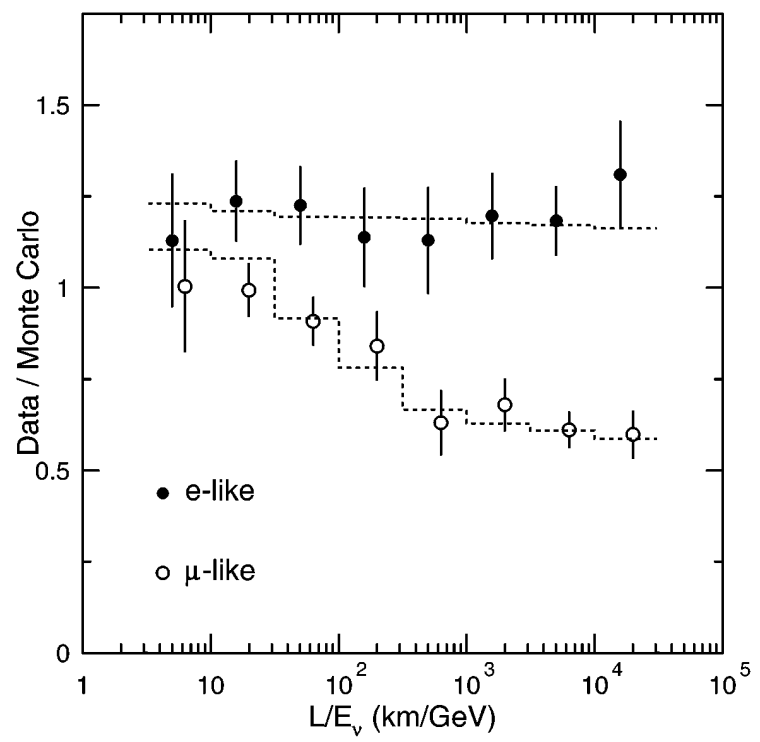
\includegraphics[width=0.5\linewidth]{superk_l_over_e.png}}%
		\subfloat[Oscillation Measurement from \cite{SuperK-Oscillations}]{
			\label{fig:superk_oscil}
			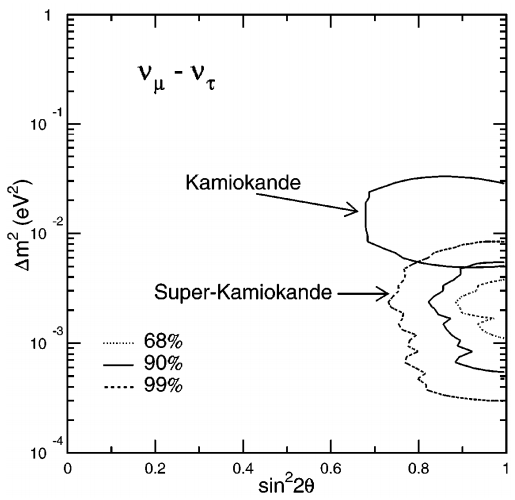
\includegraphics[width=0.5\linewidth]{superk_discovery.png}}%
	\caption{The first atmospheric neutrino oscillation measurements from the Super-K experiment. (a) The $\nu_e$-like events show no shape in L/E, as expected from a lack of neutrino oscillations. The $\nu_\mu$-like interactions, however, show a clear drop, indicating the presence of oscillation effects. (b) Using the two neutrino approximation, Super-K produced contours of the best-fit oscillation parameters for $\nu_\mu\rightarrow\nu_\tau$ oscillations. Both figures from \cite{SuperK-Oscillations}}%
\end{figure}


While investigating backgrounds, Super-Kamiokande observed an interesting deficit in the atmospheric neutrino signal.
Unlike the case in the solar neutrinos, the deficit observed by Super-K was observed solely in the muon neutrino events with no effect seem in the electron neutrinos \cite{SuperK-Oscillations}.
Using the reconstructed energy and direction of events, Super-K was able to show that the number of fully contained events of $\nu_\mu$-like interactions changed as a function of L/E - a clear signature of neutrino oscillations in the atmospheric neutrinos.
The figure, reproduced in Figure~\ref{fig:superk_l_over_e}, was used, in part, with an 2x2 approximation to the PMNS matrix to produce the first measurements, shown in Figure~\ref{fig:superk_oscil}, of the atmospheric oscillation parameters.
For the discovery of atmospheric neutrino oscillations at the same time as SNO's discovery of solar neutrino oscillations, the Super-K collaboration was jointly award the 2015 Nobel Prize \cite{NobelPrize:2015-Oscillations}.

\improvement{Add a plot of the oscillation probabilities here}


\label{subsec:global_fits}
\subsection{Global Fits to Oscillations}
Since the initial discoveries of SNO and Super-K, many experiments have measured neutrino oscillations. 
Global fits are performed and updated regularly \cite{NuFit_2.2, NuFit.org}.

The most recent results are shown in Figure~\ref{fig:nufit_v32} and include information from solar, reactor, and atmospheric oscillation experiments.
The results explicitly assume unitarity and three neutrino species.

\begin{figure}[!h]
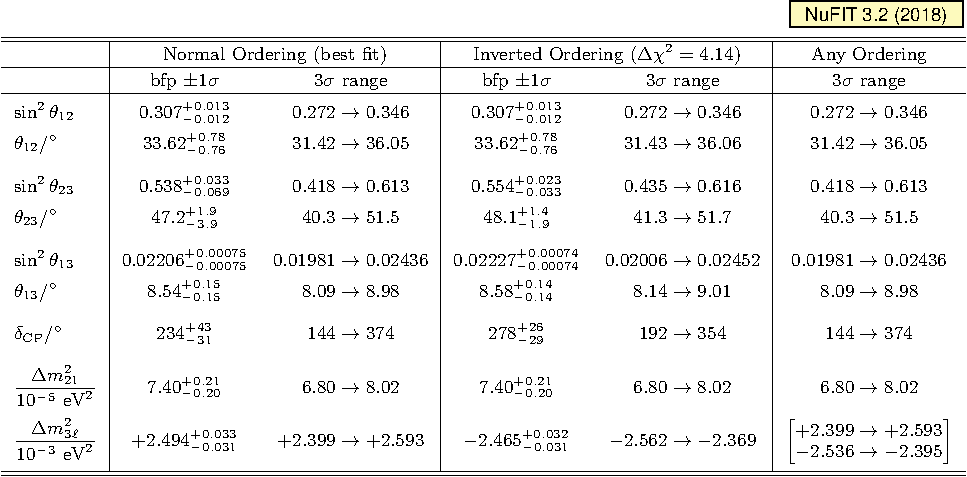
\includegraphics[width=\linewidth]{nufit_v32.pdf}
\caption{The global best-fit values for the three flavor neutrino oscillation fits as of November 2017. The first column shows results assuming the normal ordering while the second colum shows the results for the inverted ordering. Image taken from \cite{NuFit.org}}
\label{fig:nufit_v32}
\end{figure}

